 \documentclass[11pt]{article} 
\usepackage[english]{babel}
\usepackage[utf8]{inputenc}
\usepackage[margin=0.5in]{geometry}
\usepackage{amsmath}
\usepackage{amsthm}
\usepackage{amsfonts}
\usepackage{amssymb}
\usepackage[usenames,dvipsnames]{xcolor}
\usepackage{graphicx}
\usepackage[siunitx]{circuitikz}
\usepackage{tikz}
\usepackage{tkz-berge}
\usetikzlibrary{positioning, automata, backgrounds}
\usepackage[colorinlistoftodos, color=orange!50]{todonotes}
\usepackage{hyperref}
\usepackage[numbers, square]{natbib}
\usepackage{fancybox}
\usepackage{epsfig}
\usepackage{soul}
\usepackage[framemethod=tikz]{mdframed}
\usepackage[shortlabels]{enumitem}
\usepackage[version=4]{mhchem}
\usepackage{multicol}
\usepackage{forest}
\usepackage{mathtools}
\usepackage{comment}
\usepackage{enumitem}
\usepackage[utf8]{inputenc}
\usepackage{listings}
\usepackage{color}
\usepackage[numbers]{natbib}
\usepackage{subfiles}
\usepackage{tkz-berge}
\usepackage{algorithm}
\usepackage[noend]{algpseudocode}


\newtheorem{prop}{Proposition}[section]
\newtheorem{thm}{Theorem}[section]
\newtheorem{lemma}{Lemma}[section]
\newtheorem{cor}{Corollary}[prop]

\theoremstyle{definition}
\newtheorem{definition}{Definition}

\theoremstyle{definition}
\newtheorem{required}{Problem}

\theoremstyle{definition}
\newtheorem{ex}{Example}

\newcommand{\interval}[4]{\draw (#2, #1) -- (#3, #1); % Usage: \interval{height}{start}{end}{label}
\draw (#2, #1-0.11) -- (#2, #1+0.11); % draw left whisker
\draw (#3, #1-0.11) -- (#3, #1+0.11); % draw right whisker
\node[] at (#2-0.25, #1) {#4};
}


\setlength{\marginparwidth}{3.4cm}
%#########################################################

%To use symbols for footnotes
\renewcommand*{\thefootnote}{\fnsymbol{footnote}}
%To change footnotes back to numbers uncomment the following line
%\renewcommand*{\thefootnote}{\arabic{footnote}}

% Enable this command to adjust line spacing for inline math equations.
% \everymath{\displaystyle}

% _______ _____ _______ _      ______ 
%|__   __|_   _|__   __| |    |  ____|
%   | |    | |    | |  | |    | |__   
%   | |    | |    | |  | |    |  __|  
%   | |   _| |_   | |  | |____| |____ 
%   |_|  |_____|  |_|  |______|______|
%%%%%%%%%%%%%%%%%%%%%%%%%%%%%%%%%%%%%%%

\title{
\normalfont \normalsize 
\textsc{CSCI 3104 Spring 2022 \\ 
Instructors: Profs. Chen and Layer} \\
[10pt] 
\rule{\linewidth}{0.5pt} \\[6pt] 
\huge Problem Set 7\\
\rule{\linewidth}{2pt}  \\[10pt]
}
%\author{Your Name}
\date{}

\begin{document}
\definecolor {processblue}{cmyk}{0.96,0,0,0}
\maketitle


%%%%%%%%%%%%%%%%%%%%%%%%%
%%%%%%%%%%%%%%%%%%%%%%%%%%
%%%%%%%%%%FILL IN YOUR NAME%%%%%%%
%%%%%%%%%%AND STUDENT ID%%%%%%%%
%%%%%%%%%%%%%%%%%%%%%%%%%%
\noindent
Due Date \dotfill March 15 \\
Name \dotfill \textbf{Chengming Li} \\
Student ID \dotfill \textbf{109251991} \\
Collaborators \dotfill \textbf{N/A}

\tableofcontents

\section{Instructions}
{\small
 \begin{itemize}
	\item The solutions \textbf{must be typed}, using proper mathematical notation. We cannot accept hand-written solutions. \href{http://ece.uprm.edu/~caceros/latex/introduction.pdf}{Here's a short intro to \LaTeX.}
	\item You should submit your work through the \textbf{class Canvas page} only. Please submit one PDF file, compiled using this \LaTeX \ template.
	\item You may not need a full page for your solutions; pagebreaks are there to help Gradescope automatically find where each problem is. Even if you do not attempt every problem, please submit this document with no fewer pages than the blank template (or Gradescope has issues with it).

	\item You are welcome and encouraged to collaborate with your classmates, as well as consult outside resources. You must \textbf{cite your sources in this document.} \textbf{Copying from any source is an Honor Code violation. Furthermore, all submissions must be in your own words and reflect your understanding of the material.} If there is any confusion about this policy, it is your responsibility to clarify before the due date. 

	\item Posting to \textbf{any} service including, but not limited to Chegg, Reddit, StackExchange, etc., for help on an assignment is a violation of the Honor Code.

\end{itemize}}


\newpage
\section{Standard 19 - Dynamic Programming: Identify the Precise Subproblems}

\noindent The goal of this standard is to practice identifying the recursive structure. To be clear, you are \textbf{not} being asked for a precise mathematical recurrence. Rather, you are being asked to clearly and precisely identify the cases to consider. Identifying the cases can sometimes provide enough information to design a dynamic programming solution.

\subsection{Problem \ref{DP1}}
\begin{required} \label{DP1}
Consider the \textsf{Stair Climbing} problem, defined as follows.
\begin{itemize}
\item \textsf{Instance:} Suppose we have $n$ stairs, labeled $s_{1}, \ldots, s_{n}$. Associated with each stair $s_{k}$ is a number $a_{k} \geq 1$. At stair $s_{k}$, we may jump forward $i$ stairs, where $i \in \{ 1, 2, \ldots, a_{k}\}$. You start on $s_{1}$.

\item \textsf{Solution:} The number of ways to to reach $s_{n}$ from $s_{1}$.
\end{itemize}

\noindent \\ \textbf{Your job} is to clearly identify the recursive structure. That is, suppose we are solving the subproblem at stair $s_{k}$. What precise sub-problems do we need to consider?
\end{required}

\begin{proof}[Answer]
%Your answer
\begin{itemize}
\item The total steps we need to make is $n-1$ steps.
\item At the each sub problem $stair s_k $, we need to decide how many steps we want to jump. i.e $i \in \{ 1, 2, \ldots, a_{k}\}$.  The step choices at current stair $s_k$ is $\{1,2,...,a_k\}$
\item And at each sub problem $stair s_k $, we need to decide whether we jump to $s_{k+1}$ or $s_{k+2} or ...... s_{n}$
\item For example, in order to reach stair $s_6$, the steps need to take from stair 5  to 6 is 1.
\item At stair $ 4 $, the choices need to decide is 2, one choice is $4 -> 5 ->6$ and another choice is $4 -> 6$. The first path result comes from previous statement.
\item Define $T_k$ = number of steps from k to n.
\item The recurrence can be expressed as $T_k = T_{k+1} + T_{k+2} + ...+ T_{min(n,k+a_k)} + 1$ 
\end{itemize}
\end{proof}



\newpage
\subsection{Problem \ref{DP2}}
\begin{required} \label{DP2}
Fix $n \in \mathbb{N}$. The \textit{Trust Game} on $n$ rounds is a two-player dynamic game. Here, Player I starts with \$100. The game proceeds as follows.
\begin{itemize}
\item \textbf{Round 1:} Player I takes a fraction of the \$100 (which could be nothing) to give to Player II. The money Player I gives to Player II is multiplied by 1.5 before Player II receives it. Player I keeps the remainder. (So for example, if Player I gives \$20 to Player II, then Player II receives \$30 and Player I is left with \$80).

\item \textbf{Round 2:} Player II can choose a fraction of the money they received to offer to Player I. The money offered to Player I increases by a multiple of $1.5$  before Player I receives it. Player II keeps the remainder.
\end{itemize}

\noindent \\ More generally, at round $i$, the Player at the current round (Player I if $i$ is odd, and Player II if $i$ is even) takes a fraction of the money in the current pile to send to the other Player and keeps the rest. That money increases by a factor of $1.5$ before the other player receives it. The game terminates if the current player does not send any money to the other player, or if round $n$ is reached. At round $n$, the money in the pile is split evenly between the two players. \\

\noindent Each individual player wishes to maximize the total amount of money they receive. \\

\noindent \textbf{Your job} is to clearly identify the recursive structure. That is, at round $i$, what precise sub-problems does the current player need to consider? [\textbf{Hint:} Do we have a smaller instance of the Trust Game after each round?]
\end{required}

\begin{proof}[Answer]
%Your answer
\begin{itemize}
\item At each round, the player have three choices as listed below.
\item Giving all the money he has to maximize the the total amount of money he may receive if he 100 percent trusts the another player.
\item Giving some fraction of the money he has to get some profit from the multiplication if he somehow trusts the another player will pay back.
\item Giving nothing to the another player if he already satisfied the money he got.
\end{itemize}
\end{proof}




\newpage
\section{Standard 20- Dynamic Programming: Write Down Recurrences}

\subsection{Problem \ref{DP3}}

\begin{required} \label{DP3}
Suppose we have an $m$-letter alphabet $\Sigma = \{0, 1, \ldots, m-1\}$. Let $W_{n}$ be the set of strings $\omega \in \Sigma^{n}$ such that $\omega$ does not have $00$ as a substring. Let $f_{n} := |W_{n}|$. Write down an explicit recurrence for $f_{n}$, including the base cases. Clearly justify each recursive term.
\end{required}

\begin{proof}[Answer]
%Your answer here.
\begin{itemize}
\item $f_n = |W_0|  = |\Sigma^{0}| = 0$.
\item $f_1 = |W_1|  = |\Sigma^{1}| = m$. This is base case since every letter doesn't repeat. i.e. only occur once in all possible combinations.
\item $f_2 = |W_2|  = |\Sigma^{2}| = \{0, 1, \ldots, m-1\} \cdot \{1, \ldots, m-1\}= m\cdot (m-1) + (m-1).$ The "m-1" term is due to $\omega$ does not have $00$ as a substring. For the first string,\{0, 1, \ldots, m-1\}, we have m combinations. And for each combination in the first string, the second string, $\{1, \ldots, m-1\}$, can give(m-1) combinations with that. That is why we have $m\cdot (m-1)$ term as the first term. The first term only eliminates the possibility of the first $0$ occurrence. So we need to add another (m-1) term to eliminate the possibility of the second $0$ occurrence.
\item $f_3 = |W_3|  = |\Sigma^{3}| = \{0, 1, \ldots, m-1\} \cdot \{1, \ldots, m-1\} \cdot \{1, \ldots, m-1\}= (m-1)f_2 + (m-1)f_1.$ The "m-1" term is due to $\omega$ does not have $00$ as a substring.
\item Same thing apply to the general case. (m-1) is used to eliminate the possibility of $0$ occurrence. And we multiply the result to $f_{n-1}$ combinations, which we already known the solution of W that doesn't have substring $00$. And same rule apply to the result to $f_{n-2}$ combinations.
\end{itemize}

\begin{align*}
f_{n} &= \begin{cases} \text{0} & : \text{n = 0}, \\ 
\text{m} & : \text{n = 1},\\
\text{$f_1\cdot (m-1) + (m-1)$} & : \text{n = 2}.,\\
\text{$f_{n-1}\cdot (m-1) + f_{n-2}\cdot(m-1)$} & : \text{$n \geq 3$}.,\\
\end{cases}
\end{align*}
\end{proof}

%You may find the following commented code helpful in rendering a recurrence
\begin{comment}
\begin{align*}
f_{n} &= \begin{cases} \text{Case1} & : \text{Condition1}, \\ 
\text{Case2} & : \text{Condition2}. 
\end{cases}
\end{align*}
\end{comment}




\newpage
\subsection{Problem \ref{DP4}}

\begin{required} \label{DP4}
Suppose we have the alphabet $\Sigma = \{x, y\}$. For $n \geq 0$, let $W_{n}$ be the set of strings $\omega \in \{x, y\}^{n}$ where $\omega$ contains $yyy$ as a substring. Let $f_{n} := |W_{n}|$. Write down an explicit recurrence for $f_{n}$, including the base cases. Clearly justify each recursive term.
\end{required}

\begin{proof}[Answer]
%Your answer here.
\begin{itemize}
\item $F_n = |W_0|  = |\Sigma^{0}| = 0$.
\item $F_1 = |W_1|  = |\Sigma^{1}| = 2$. This is base case since every letter doesn't repeat. i.e. only occur once in all possible combinations.
\item $F_2 = |W_2|  = |\Sigma^{2}| = 2*2$
\item $F_3 = |W_3|  = |\Sigma^{3}|$ = $(2-1)\cdot F_2 + (2-1)\cdot F_1 + (2-1) $ 
\item the term (2-1) is used to eliminate the possibility of $y$ occurrence. $F_2$ with (2-1) term is used to eliminates the possibility of first $y$ occurrence. $F_1$ with (2-1) is used to eliminates the possibility of second $y$ occurrence. (2-1) term is used to eliminates the possibility of third $y$ occurrence.

\item $F_n = |W_n|  = |\Sigma^{n}|$ = $(2-1)\cdot F_{n-1} + (2-1)\cdot F_{n-2} + (2-1)\cdot F_{n-3} $ 
\item the term (2-1) is used to eliminate the possibility of $y$ occurrence. $F_{n-1}$ with (2-1) term is used to eliminates the possibility of first $y$ occurrence. $F_{n-2}$ with (2-1) is used to eliminates the possibility of second $y$ occurrence. $F_{n-3}$ with (2-1) term is used to eliminates the possibility of third $y$ occurrence.
\end{itemize}

\begin{align*}
F_{n(noyyy)} &= \begin{cases} \text{0} & : \text{n = 0}, \\ 
\text{2} & : \text{n = 1},\\
\text{4} & : \text{n = 2},\\
\text{$(2-1)\cdot F_2 + (2-1)\cdot F_1 + (2-1) $} & : \text{n = 3},\\
\text{$(2-1)\cdot F_{n-1} + (2-1)\cdot F_{n-2} + (2-1)\cdot F_{n-3} $ } & : \text{$n \geq 4$}.,\\
\end{cases}
\end{align*}

\begin{itemize}
\item $f_n$ have $2^n$ combinations. Above, I find the number of string that doesn't contain $yyy$ as a substring.  Then $2^n- F_n$ is the number of string that does contain $yyy$ as a substring.
\item $2^n = F_n + f_n$. So $ F_n = 2^n - f_n$
\end{itemize}
\begin{align*}
f_{n(yyy)} &= \begin{cases} \text{0} & : \text{n = 0}, \\ 
\text{0} & : \text{n = 1},\\
\text{0} & : \text{n = 2},\\
\text{1} & : \text{n = 3},\\
\text{$2^n - F_{n(noyyy)}$ } & : \text{$n \geq 4$}.,\\
\end{cases}
\end{align*}

\begin{align*}
f_n &= 2^n - F_n\\
&= 2^n - F_{n-1}- F_{n-2}- F_{n-3}\\
&= 2^n - (2^{n-1}-f_{n-1})- (2^{n-2}-f_{n-2})- (2^{n-3}-f_{n-3})\\
&= 2^n(1-1/2-1/4-1/8) + f_{n-1} + f_{n-2} + f_{n-3}\\
&= 2^n \cdot 1/8 + f_{n-1} + f_{n-2} + f_{n-3}\\
&= 2^{n-3}+ f_{n-1} + f_{n-2} + f_{n-3}
\end{align*}
\end{proof}

\begin{align*}
f_{n(yyy)} &= \begin{cases} \text{0} & : \text{n = 0}, \\ 
\text{0} & : \text{n = 1},\\
\text{0} & : \text{n = 2},\\
\text{1} & : \text{n = 3},\\
\text{$2^{n-3}+ f_{n-1} + f_{n-2} + f_{n-3}$ } & : \text{$n \geq 4$}.\\
\end{cases}
\end{align*}



\newpage
\section{Standard 21- Dynamic Programming: Using Recurrences to Solve}

\subsection{Problem \ref{Recurrence1}}
\begin{required} \label{Recurrence1}
Given the following directed acyclic graph. Use dynamic programming to fill in a \textbf{one-dimensional} lookup table that counts number of paths from each node $j$ to 14, for $j \geq 1$. Note that a single vertex is considered a path of length $0$. \textbf{Fill in the lookup table for all vertices 1-14; and in addition, clearly show work for vertices 9-14}.

        % ----- FIGURE -----
        \begin{figure}[h!]
        \begin{center}
        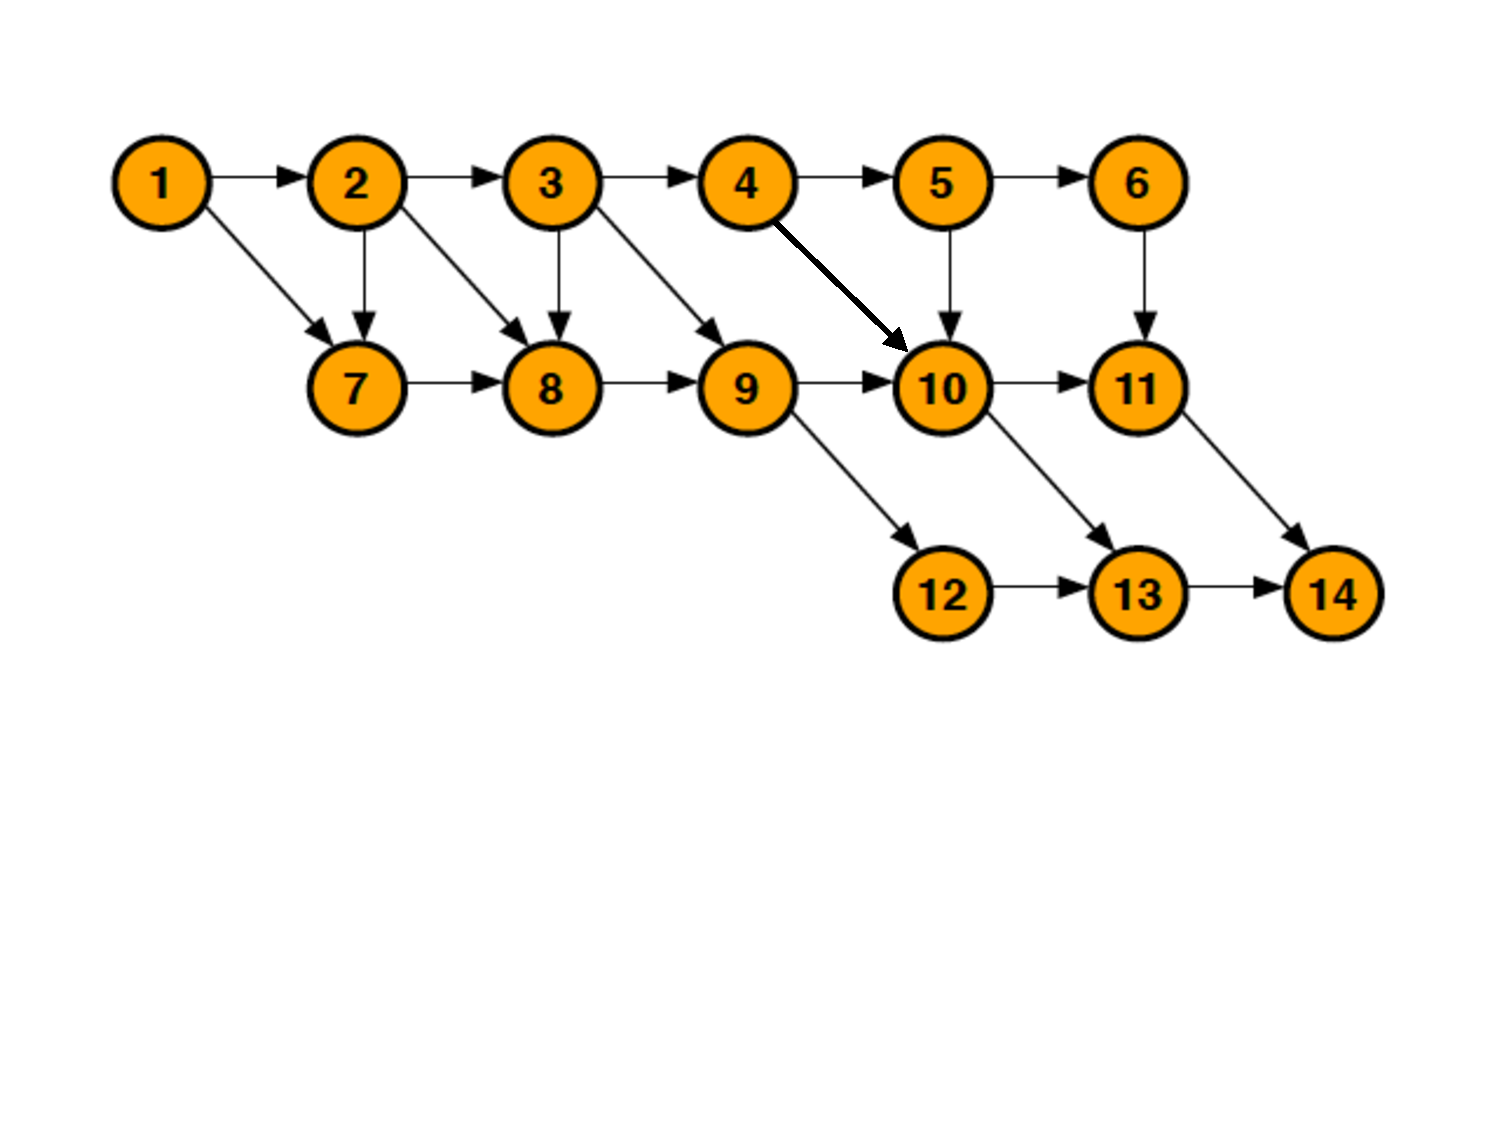
\includegraphics[scale=0.45]{dag_ps10.pdf} 
        \end{center}
        \end{figure}
        % ----------

\end{required}


\begin{proof}[Answer]
%Your answer
\textbf{Define expression:\\}
\textbf{(1,14) = number of paths from node 1 to 14\\}
\textbf{Example: (11,14) = 1; (10,14) = (11,14) + (13,14) = 1 + 1}
\begin{center}
\begin{tabular}[c]{c|c|c} 
From& To 14 & result \\\hline
1 & (2,14) + (7,14) = 17 + 3 & 20\\
2 & (3,14) + (7,14) + (8,14) = 11+3+3 & 17\\
3 & (4,14) + (8,14) + (9,14) = 5 + 3 + 3 & 11\\
4 & (5,14) + (10,14) = 3 + 2 & 5\\
5 & (10,14) + (6,14) = 2 + 1 & 3\\
6 & (11,14) & 1\\
7 & (8,14) & 3\\
8 &	(10,14) + (12,14) = 2 + 1 & 3\\
9 &  (10,14) + (12,14) = 2 + 1  &3\\
10 &  (11,14) + (13,14)  &2\\
11 & 1&1\\
12 & 1&1\\
13 & 1&1\\
14 & 1&1
\end{tabular}
\end{center}	

\begin{itemize}
\item At vertex 14, there is 0 path from 14 to 14
\item At vertex 13, there is 1 path from 13 to 14. i.e. $13->14$
\item At vertex 12, there is 1 path from 12 to 14. i.e $12->13->14$
\item At vertex 11, there is 1 path from 11 to 14. i.e. $11->14$
\item At vertex 10, there are two branches. path1: $11->14$. path2: $13->14$. So 2 paths from 10 to 14.
\item At vertex 9, there are two branches. path1: $10->14$. path2: $12->14$. Path1 result can be found from vertex 10 and path2 result can be found from vertex 12. So, 3 paths from 9 to 14.
\end{itemize}
\end{proof}




\newpage
\subsection{Problem \ref{Recurrence2}}
\begin{required} \label{Recurrence2}
Consider the following input for the Knapsack problem with a capacity $W=12$:\\

 \begin{tabular}{r|c|c|c|c|c|c}
        item $i$  & 1  & 2 &3 &4 &5 &6 \\
                \hline
        value $v_i$ &2 & 7& 18&23 &29 &35 \\
          \hline
        weight $w_i$ & 1 & 2  & 5& 6& 7& 9\\
                 \end{tabular}

\vspace{1mm}
\noindent \\ 
Fill in a lookup table, similar to the example on page 12 of course notes for week 9 (see Week 9 under ``Modules" of the course canvas). In addition, clearly explain how you obtain the maximum values/profits $OPT(6, w)$, $w=7,~8,~9,~10,~11,~12$.

\end{required}

\begin{proof}[Answer]
%Your answer here
\begin{tabular}{r|c|c|c|c|c|c|c|c|c|c|c|c|c}
          	  &0& 1  & 2 &3 &4 &5 &6&7 &8 &9&10&11&12 \\\hline
	 \{\}  & 0  & 0 &0 &0 &0 &0&0 &0 &0 &0&10&11&12\\\hline
                
       \{1\}  & 0  & 2 &2 &2 &2 &2& 2& 2& 2&2&2&2&2\\\hline
         
        \{1,2\}  & 0  & 7 &9 &9 &9 &9&9 &9 &9 &9&9&9&9\\\hline

        \{1,2,3\}  & 0  & 2 &7 &9 &9 &18&20 &25 &27 &27&27&27&27\\\hline

        \{1,2,3,4\}  & 0  & 2 &7 &9 &9 &18&23 &25 &30 &32&32&41&43\\\hline

       \{1,2,3,4,5\}  & 0  & 2 &7 &9 &9 &18&23 &29 &31 &36&38&41&47\\\hline

        \{1,2,3,4,6\}  & 0  & 2 &7 &9 &9 &18&23 &29 &31 &36&38&42&47\\\hline

\end{tabular}
\begin{itemize}
\item In OPT(i,w), i refers to row i in the table, w refers to column w in the table

\item OPT(6,7): $w_6=9 > 7.$So, OPT(6,7) = OPT(5,7) = 29.\\
To obtain OPT(6,7), we know $w_6 = 9>7$ . So we need to \textbf{pick OPT(i-1=5,7)},based on Knapspack algorithm, which comes from row 5 and column 7 with value 29.

\item OPT(6,8): $w_6=9 > 8.$So, OPT(6,7) = OPT(5,8) = 31\\
To obtain OPT(6,8), we know $w_6 = 9>8$ . So we need to \textbf{pick OPT(i-1=5,8)},based on Knapspack algorithm, which comes from row 5 and column 8 with value 31.

\item OPT(6,9): $w_6 =9 =9.$So max(OPT(5,9), $v_6$ + OPT(5,9-9)) = max(36,35+0) = 36\\
 To obtain OPT(6,9), we know $w_6 = 9=9$ . So, based on the algorithm, we need to decide $max(OPT(6-1=5,9), v_6 + OPT(6-1=5, w-w_6 = 9-9=0))$.\textbf{I will pick the OPT(5,9) from the table as solution.} The result is $max(OPT(5,9), v_6 + OPT(5, 0)) =  36$

\item OPT(6,10):$w_6 =9 < 10.$So, max(OPT(5,10), $v_6$ + OPT(5,10-9)) = max(38,35+2) = 38
\\To obtain OPT(6,10), we know $w_6 = 9<10$ . So, based on the algorithm, we need to decide $max(OPT(6-1=5,10), v_6 + OPT(6-1=5, w-w_6 = 10-9=1))$.\textbf{I will pick the OPT(5,10) from the table as solution.} The result is $max(OPT(5,10), v_6 + OPT(5, 1)) =  38$

\item OPT(6,11):$w_6 =9 < 11.$So, max(OPT(5,11), $v_6$ + OPT(5,11-9)) = max(41,35+7 = 42) = 42
\\ To obtain OPT(6,11), we know $w_6 = 9<11$ . So, based on the algorithm, we need to decide $max(OPT(6-1=5,11), v_6 + OPT(6-1=5, w-w_6 = 11-9=2))$.\textbf{I will pick the $v_6$ + OPT(5,2) = 42 from the table as solution.} The result is $max(OPT(5,11), v_6 + OPT(5, 2)) =  42$

\item OPT(6,12):$w_6 =9 < 12.$So, max(OPT(5,12), $v_6$ + OPT(5,12-9)) = max(47,35+9 = 44) = 47
\\ To obtain OPT(6,12), we know $w_6 = 9<12$ . So, based on the algorithm, we need to decide $max(OPT(6-1=5,12), v_6 + OPT(6-1=5, w-w_6 = 12-9=3))$.\textbf{I will pick the OPT(5,12) from the table as solution.} The result is $max(OPT(5,12), v_6 + OPT(5, 3)) =  47$
\end{itemize}
\end{proof}

\end{document} % NOTHING AFTER THIS LINE IS PART OF THE DOCUMENT



